\documentclass[iutinfo,a4paper,nocorrections,10pt]{ustl-tdtp}
%\usepackage[utf8]{inputenc}  
%\usepackage[T1]{fontenc}
\usepackage{listings}  
\usepackage{version}
\usepackage{subcaption}

%\usepackage[a4paper]{geometry}


\etablissement{\ustl}
\formation{DUT info 2ème année}
\matiere{Structures de données}
\titre{TD 2 : Listes chaînées}
\date{\annee{2018}--\annee{2019}}
%\enseignant{}

%\includeversion{solution}
%\excludeversion{solution}

\newcommand{\case}{}%\rule[-.40cm]{0pt}{1cm}}
\newcommand{\ident}[3]{(\texttt{#1},~\texttt{#2},~\texttt{#3})}
\newcommand{\rien}{}

\parindent 0cm
\begin{document}
\maketitle
\thispagestyle{empty}



La première partie du TD concerne l'écriture des méthodes de bases d'insertion, de suppression et de parcours de listes chaînées représentées sous forme de maillons. La deuxième partie est consacrée aux itérateurs. La troisième partie aborde les listes chaînées sous la forme de structure récursive. Vous utiliserez la syntaxe Java.


\section{Les listes chaînées : représentation sous forme de maillons}

\subsection{Qu'est-ce qu'une liste chaînée?}

Une liste chaînée correspond à un assemblage d'éléments (ou maillons) reliés entre eux pour former une chaîne. Dans sa version simple, chacun des maillons contient une partie qui correspond aux données que l'on souhaite enregistrer dans la liste et une référence vers le maillon suivant dans la liste. Ainsi, contrairement à un tableau qui correspond à des cases contiguës en mémoire, il n'y a pas de localité spatiale entre les éléments. On passe d'un maillon à un autre grâce à des références. Les maillons peuvent se trouver à des endroits très différents en mémoire.

\begin{figure}[!h]
\centering
\label{tableau}
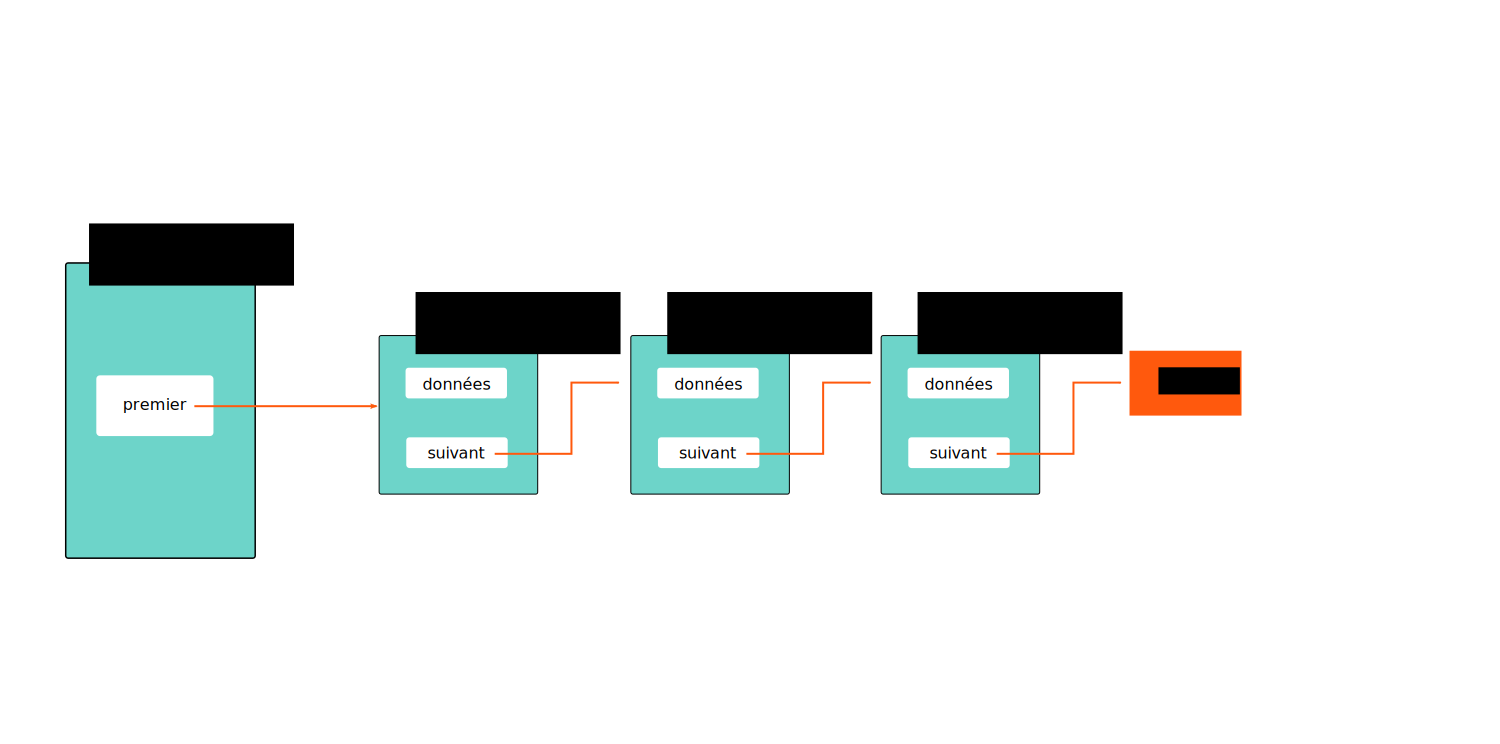
\includegraphics[scale=0.5]{figs/linked_list}
\caption{}
\end{figure}

\subsection{Conception orientée objet}

\question En vous inspirant du schéma, proposez une modélisation objet d'une liste chaînée. Nous considérerons que les données d'un maillon représentent une chaîne de caractères \texttt{nom}. Écrivez les constructeurs associés.


\begin{correction}
{\color{red}
\begin{lstlisting}[language=Java]
public class ListeChainee{

    Maillon premier;
    
    public ListeChainee(){
	this.premier = null;
    } 
    
    private class Maillon{
	
	private int cle;
	private String nom;
	Maillon suivant;
	
	public Maillon(int cle, String nom){
	this.cle = cle;
	this.nom = nom;
	this.suivant = null;	
	} 
    }
}
\end{lstlisting}
}

\end{correction}




\question Modifiez vos classes de manière à obtenir une liste générique.


\begin{correction}
{\color{red}
\begin{lstlisting}[language=Java]
public class ListeChainee<E>{
 
    private Maillon premier;
    
    public ListeChainee(){
	this.premier = null;
    } 

    private class Maillon{
	
	public  E valeur;
	public Maillon suivant;
	
	public Maillon(E valeur){
	    this.valeur = valeur;
	    this.suivant = null;	
	} 
   }
}
\end{lstlisting}
}

\end{correction}

\question Écrivez une méthode \texttt{public boolean estVide()} qui indique si la liste est vide ou non.

\question Écrivez une méthode \texttt{public void ajoute(E valeur)} qui ajoute l'objet valeur en tête de liste.

\question Écrivez une méthode \texttt{public E supprimePremier()} qui supprime l'objet valeur en tête de liste et le retourne. 

\question Écrivez une méthode \texttt{public void affiche()} qui affiche la liste chaînée.

%\question Écrivez maintenant la méthode \texttt{public void supprime(E valeur)} qui supprime l'objet valeur dans la liste.

\begin{correction}
{\color{red}
\begin{lstlisting}[language=Java]
public class ListeChainee<E>{

    private Maillon premier;
    
    public ListeChainee(){
	 this.premier = null;
    } 
    
    public boolean estVide(){
	  return this.premier == null;
    }
    
    public void ajoute(E valeur){
	  Maillon m = new Maillon(valeur);
	  m.suivant = premier;
	  this.premier = m; 
    }
    
    public E supprimePremier(){
	  Maillon tmp = premier;
	  premier = premier.suivant;
	  return tmp.valeur;
    }
    
    public void affiche(){
	  Maillon current = premier;
	  while(current!=null){
	    System.out.println(current.valeur);
	    current = current.suivant;
	  }
    } 
}
\end{lstlisting}
}

\end{correction}

\section{Les itérateurs}
\subsection{Qu'est-ce qu'un itérateur?}
Un itérateur est un \textit{curseur} que l'on peut déplacer sur les maillons d'une liste. L'itérateur peut réaliser les opérations suivantes :

\begin{itemize}
\item[•] Se déplacer d'un élément vers la droite via la méthode \texttt{next()} 
\item[•] Vérifier s'il est possible de se déplacer d'un élément vers la droite via la méthode \texttt{hasNext()}. 
\end{itemize}

~


\begin{figure}[ht!]
 \begin{subfigure}[b]{0.45\textwidth}
                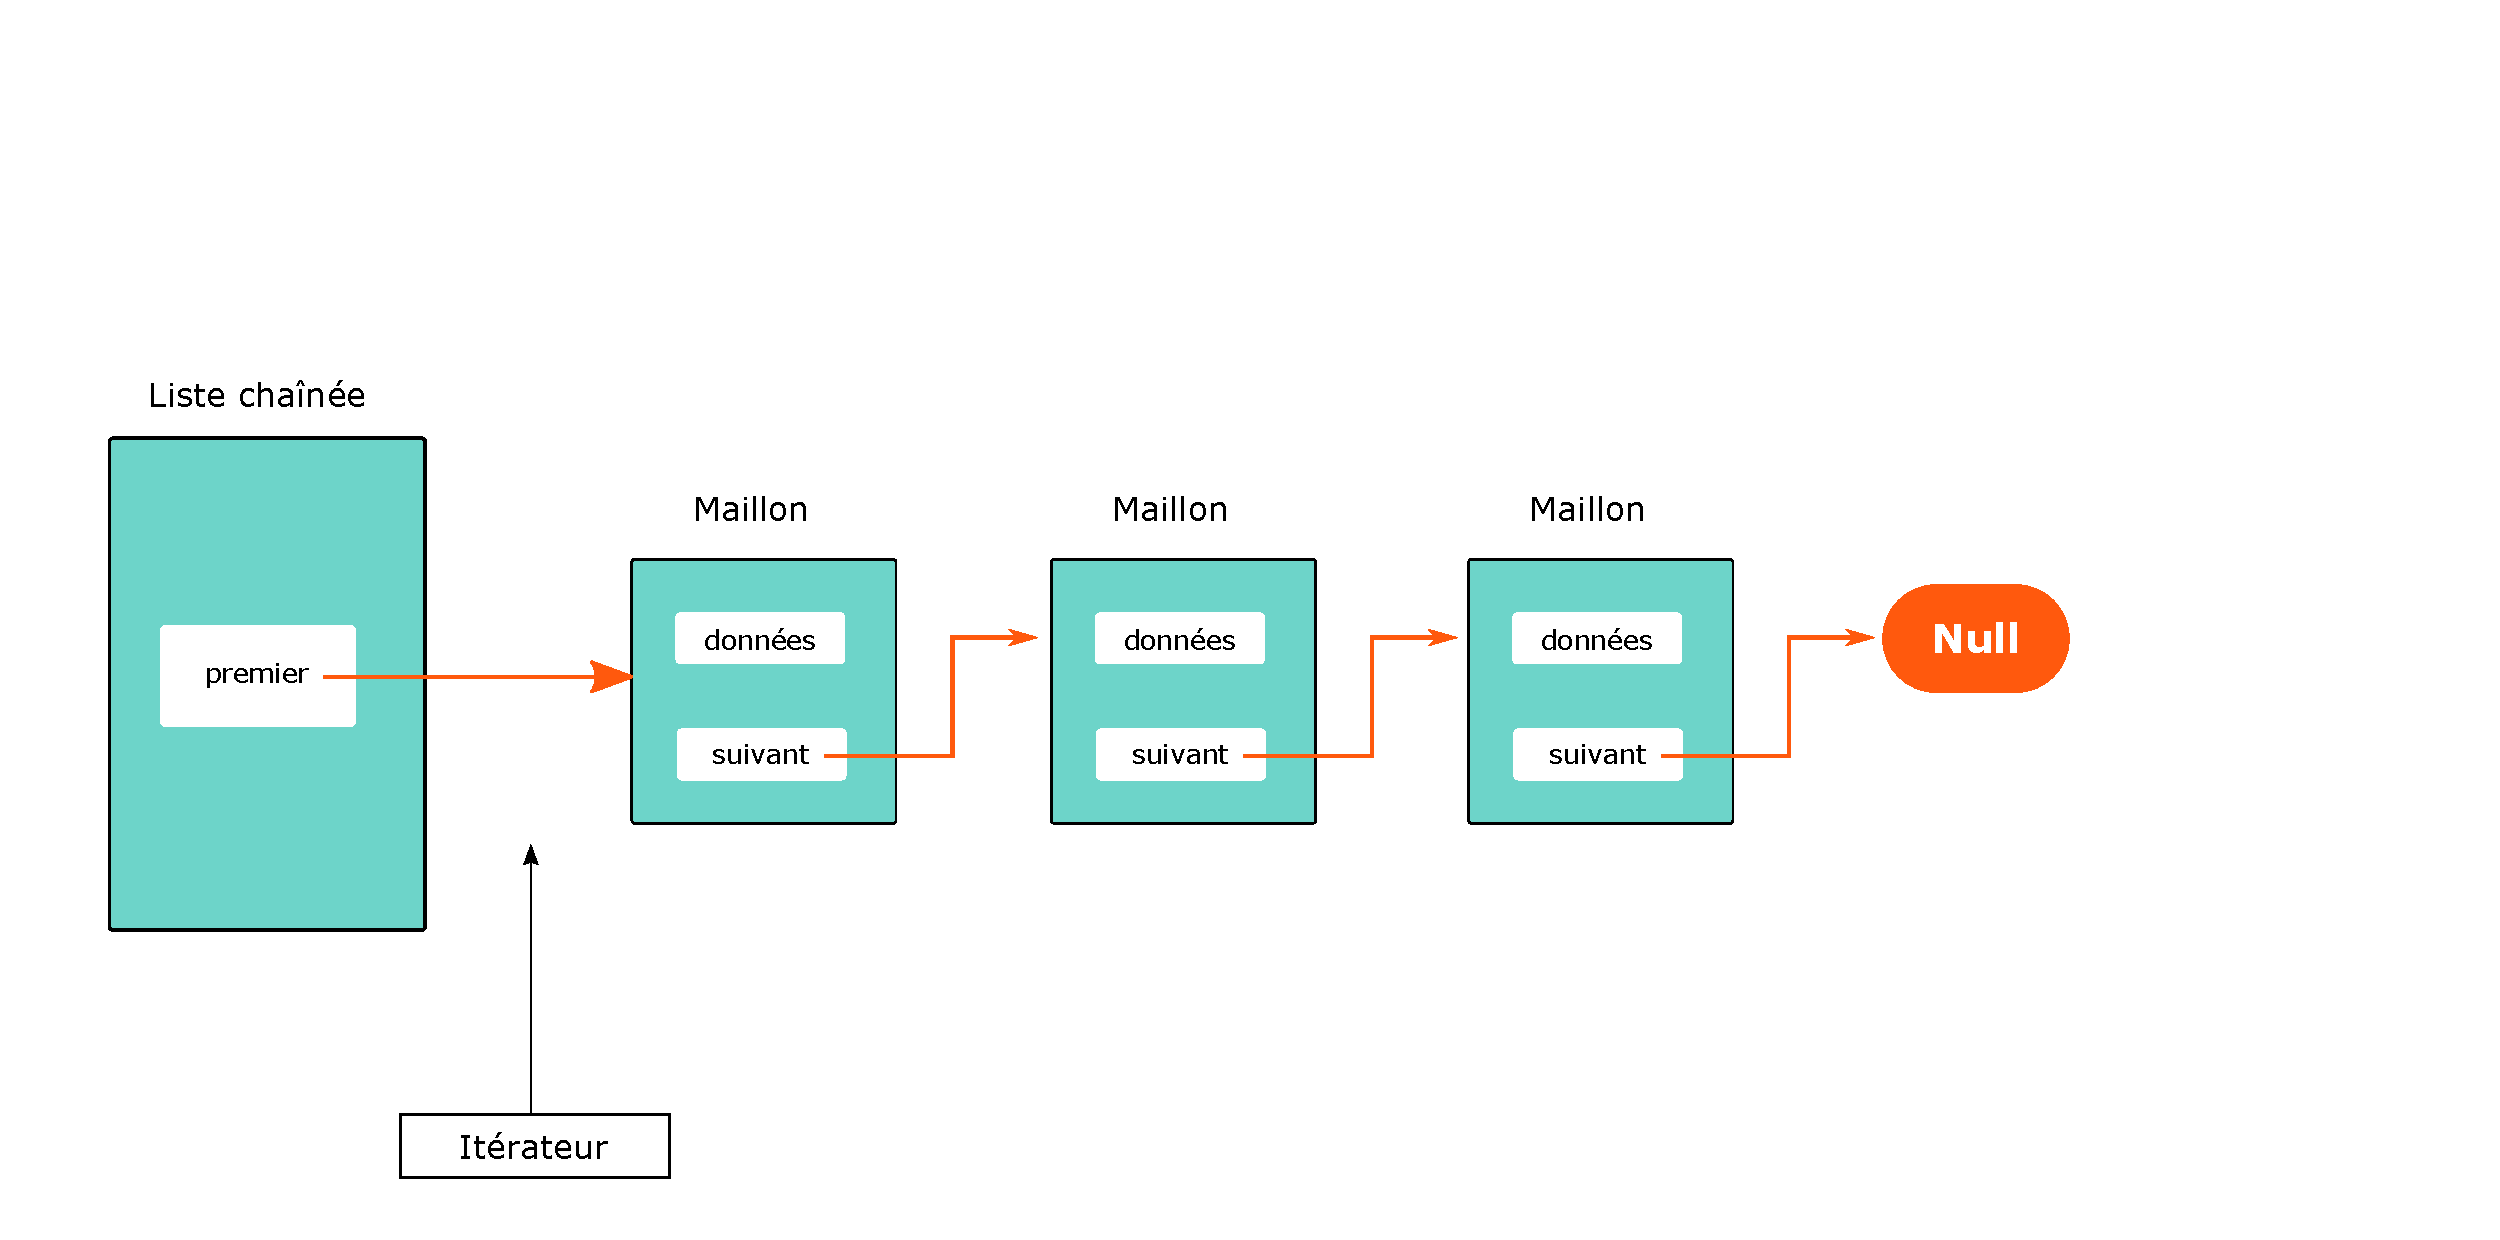
\includegraphics[width=\textwidth]{figs/linked_list_ite}
                \caption{Position initiale de l'itérateur}
                \label{fig:ite1}
        \end{subfigure}%
        \hfill
        ~ %add desired spacing between images, e. g. ~, \quad, \qquad, \hfill etc.
          %(or a blank line to force the subfigure onto a new line)
        \begin{subfigure}[b]{0.45\textwidth}
                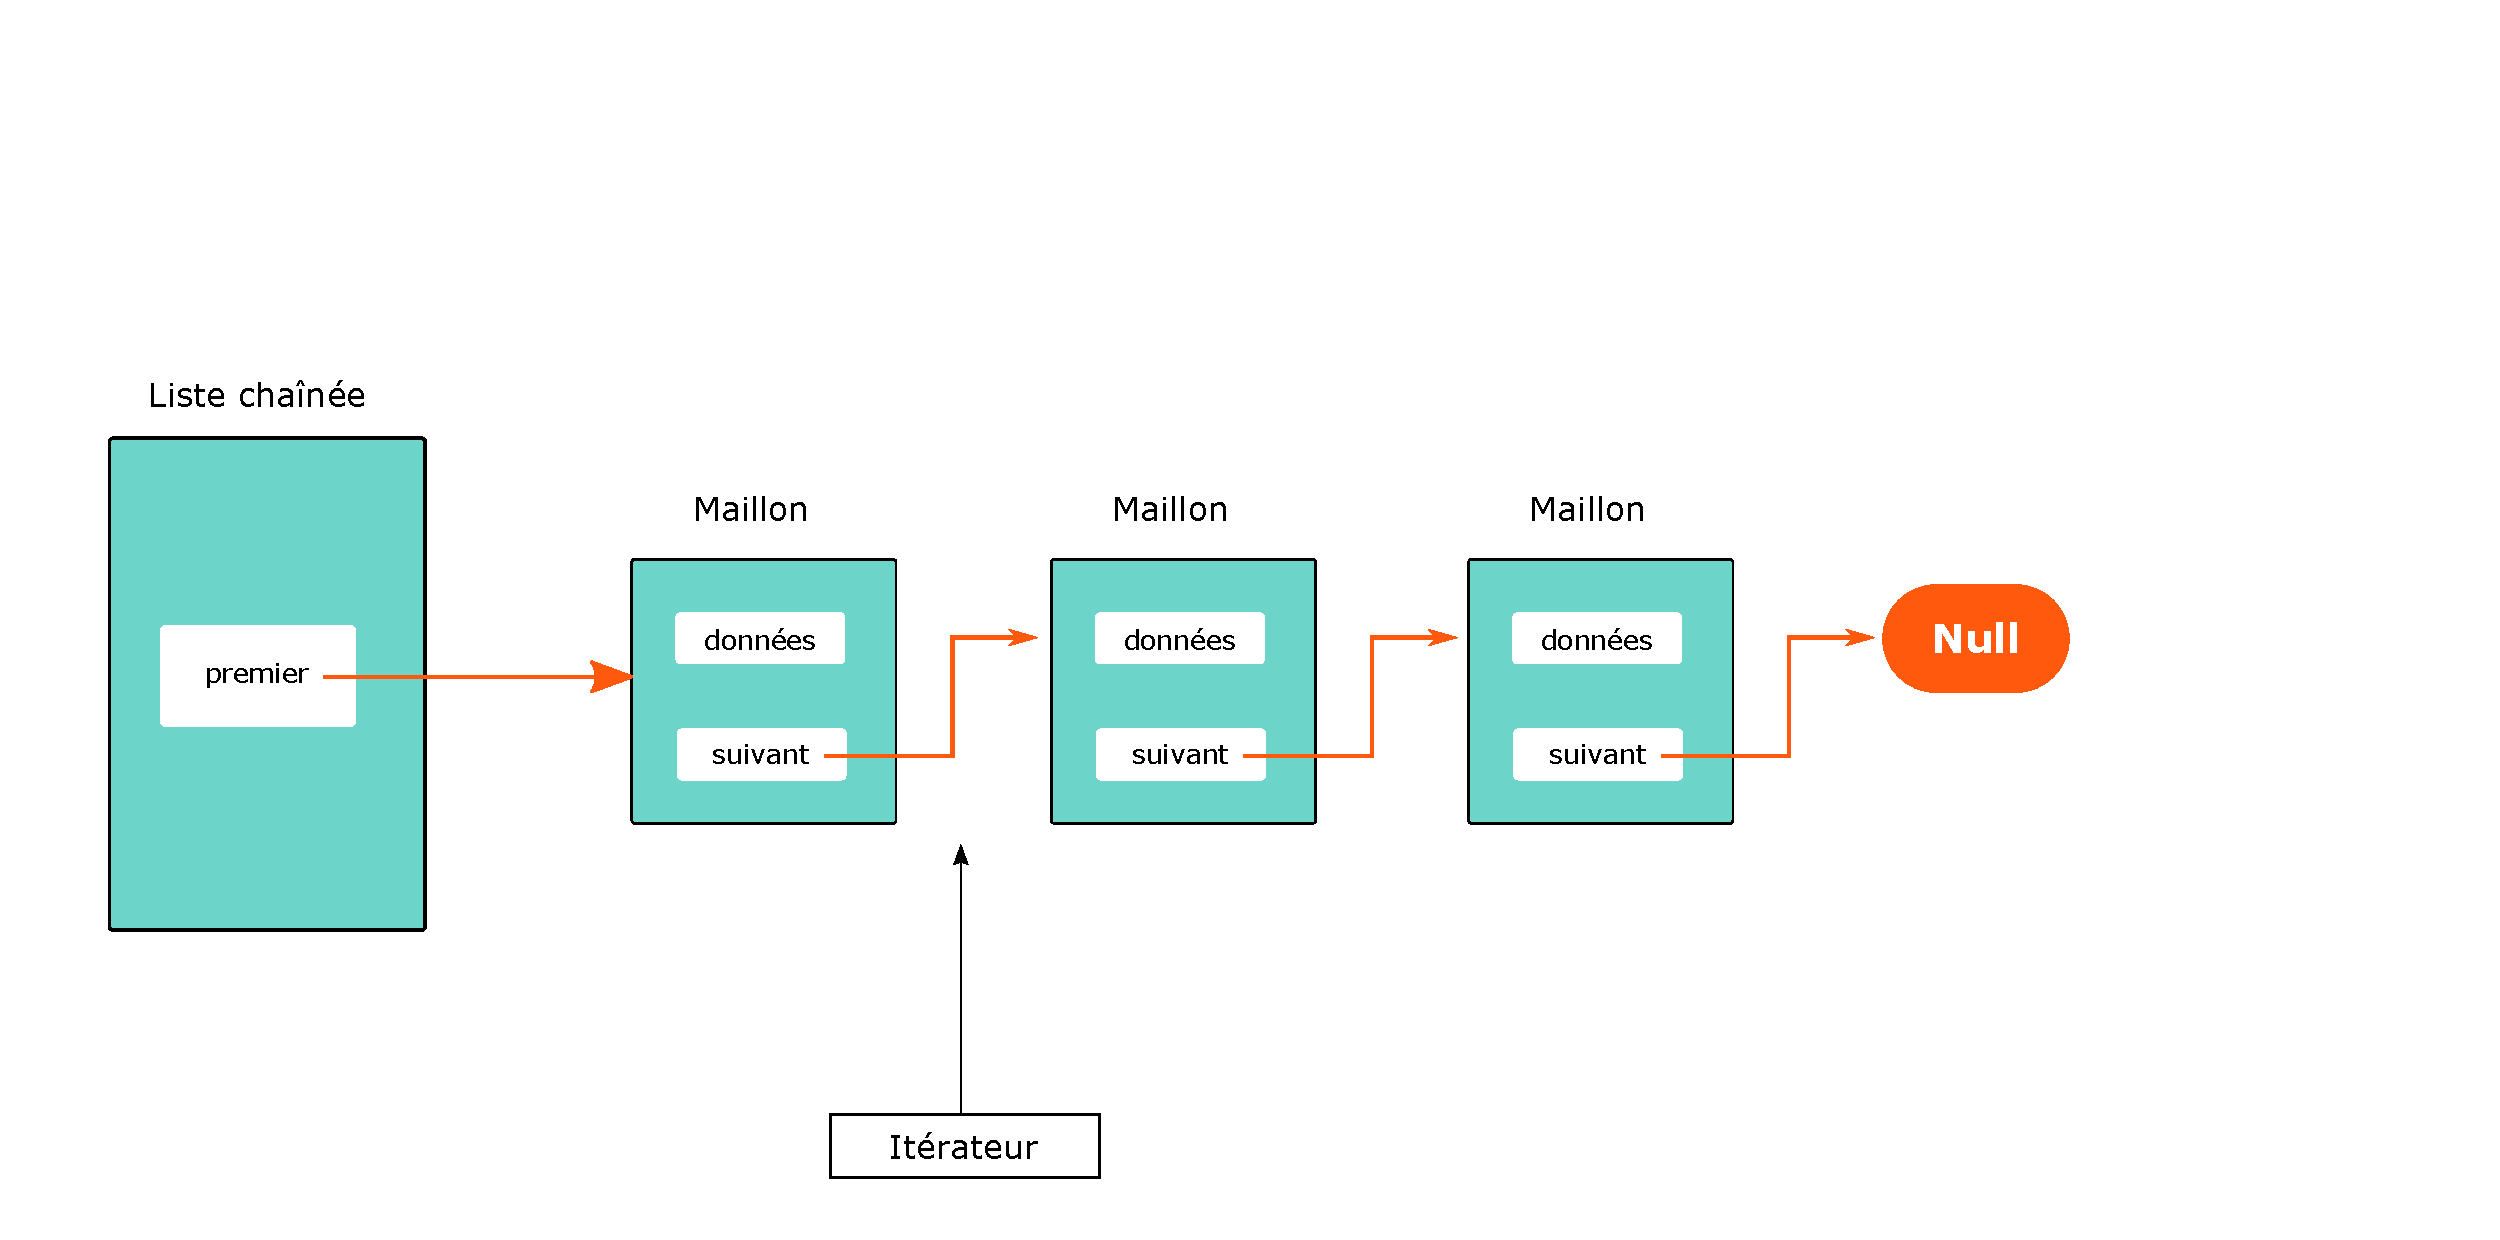
\includegraphics[width=\textwidth]{figs/linked_list_ite2}
                \caption{Position de l'itérateur après un appel à \texttt{next()}}
                \label{fig:ite2}
        \end{subfigure}
\caption{Un itérateur}

\label{fig:ite}


\end{figure}


\textbf{Remarque 1} : Comme indiqué en Figure~\ref{fig:ite1}, à l'état initial l'itérateur est positionné avant le premier élément de liste. Un premier appel à \texttt{next()} est alors nécessaire pour que l'itérateur pointe sur le premier objet de la liste.\newline

\textbf{Remarque 2} : Il est tout à fait possible de déclarer plusieurs itérateurs sur une même liste.\newline

\question Écrivez une classe \texttt{MyIterator<T>} qui implémente \texttt{Iterator<T>} et permettra d'itérer sur la liste déjà implémentée.

\question Écrivez la méthode \texttt{boolean hasNext()} qui retourne vrai s'il est possible de déplacer le curseur à droite.\newline

\question Écrivez la méthode \texttt{E next()} qui déplace le curseur vers la la droite de la liste et retourne l'élément "pointé" par le curseur ou \texttt{null} le cas échéant.\newline

\question Rendez maintenant votre classe \texttt{Iterable<T>} et implémentez la méthode \texttt{Iterateur<T> iterateur()} qui retourne un itérateur associé à la liste.\newline




\begin{correction}
{\color{red}
\begin{lstlisting}[language=Java]

public class ListeChainee<E>{

   public Iterateur getIterateur(){
	return new Iterateur();
    }

    private class Iterateur{
   	
   	private Maillon curseur;
   	
   	public Iterateur(){
	    this.curseur=null;
   	}
   	
   	public boolean hasNext(){
	    if(ListeChainee.this.estVide()){ 
		//Si instance de ListeChainee associee a l'iterateur est vide
		return false;	    	  
	    }else{
		if(this.curseur==null) //Liste non vide mais curseur avant premier maillon
		    return true; 	
		return (this.curseur.suivant!=null);
        }
    }   
	
    public E next(){
      if(!hasNext()) return null;//ou mieux une exception
      
      if(this.curseur==null){
        this.curseur=ListeChainee.this.premier;
      }else this.curseur=curseur.suivant;
        return this.curseur.valeur;
       
    }
  }
}


\end{lstlisting}
}

\end{correction}

\section{Une représentation récursive}
\subsection{Une structure récursive par nature}

Une liste peut être définie récursivement par :
\begin{itemize}
\item[-]Soit la liste est vide,
\item[-]Soit elle est un élément suivi d'une liste.
\end{itemize}
~
\question Écrivez une méthode récursive \texttt{boolean contains(Object o)} qui retourne vrai si la liste contient l'objet \texttt{o}, faux autrement. 

\begin{correction}
{\color{red}
\begin{lstlisting}[language=Java]
 boolean contains(Object o){
   if(value == null) return false;
   if(value.equals(o))return true;
   return contains(suivant,o);
 }
\end{lstlisting}
}
\end{correction}


\question Écrivez une méthode récursive \texttt{int length()} qui retourne la taille de la liste de premier maillon m.

\begin{correction}
{\color{red}
\begin{lstlisting}[language=Java]
 int length(){
   if(value == null) return 0;
   return 1 + length(m.suivant);
 }
\end{lstlisting}
}
\end{correction}

\question Votre méthode est-elle récursive terminale? Sinon proposez-en une. 

\begin{correction}
{\color{red}
\begin{lstlisting}[language=Java]
 int length(Maillon m){
   return lengthAux(m, 0);
 }
 int lengthAux(Maillon m, int cpt){
   if(m == null) return 0;
   return lengthAux(m.suivant, cpt+1);
 }
\end{lstlisting}
}
\end{correction}

\question Écrivez une méthode récursive \texttt{void afficheEnvers()} qui affiche la liste à l'envers.

\begin{correction}
{\color{red}
\begin{lstlisting}[language=Java]
 void afficheEnvers(Maillon m){
   if(m == null) return ;
   afficheEnvers(m.suivant);
   System.out.println(m.value);

 }
\end{lstlisting}
}
\end{correction}

\end{document}

